%!TEX root = ./report.tex

\section{Linearization, Discretization and Simulation}
In this first part of the case study. The given system model of the path tracking system is analyzed and simulated.
Therefore, the system will be linearized and discretized. 
As a nominal trajectory is required for the linearization, these will be computed first.
In the end of this first part, simulation results of the simulated non-linear system, the linearized system and a dicretized linear system will be compared.

\subsection{Nominal Trajectories}
First, a nominal trajectory is computed.
A nominal trajectory is a function of the state variables and the input variable of time.
The nominal trajectories are a solution of the system model.

In order to obtain a nominal trajectory some contraintes are added to the state space equations.
It is assumed that the vehicle perfectly follows the desired trajectory.
Therefore, the lateral deviation and the heading error are zero and stay zero among all times.
Further, a constant speed is assumed.
Using these assumptions several contraints are added to the state space model.
Table~\ref{tab:nominal_contraints} summarizes the constraints.
\begin{table}[h]
	\centering
	\begin{tabular}{c|l}
	\hline
	\hline
	\textbf{Constraint} & \textbf{Description}\\
	\hline
	$\bar{x}_2 = 0$\\$\bar{\dot{x}}_2 = 0$ & no lateral deviation\\\hline
	$\bar{x}_3 = 0$\\$\bar{\dot{x}}_3 = 0$& no heading error\\\hline
	$\bar{x}_4 = v_{ref}$\\$\bar{\dot{x}}_4 = 0$& constant speed\\\hline
	$\bar{\dot{x}}_5 = 0$ & steering wheel actuator is at steady state\\
	\hline
	\end{tabular}
	\caption{Contraints for the nominal trajectory.}
	\label{tab:nominal_contraints}
\end{table}

\noindent Using \eqref{eq:ss1} we obtain
\begin{equation}
	\bar{\dot{x}}_1 = v_{ref} \Rightarrow \bar{x}_1 = v_{ref} \cdot t
\end{equation}
and using \eqref{eq:ss3}
\begin{equation}
	0 = \frac{v_{ref}}{L} \tan(\bar{x}_5) - \kappa v_{ref} \Rightarrow \bar{x}_5 = \arctan (\kappa L) \, .
\end{equation}
Further, using the actuator equations \eqref{eq:ss4} and \eqref{eq:ss5} the control input can be computed.
Finally, the resulting nominal trajectory for the state $\bar{x}$ is
\begin{eqnarray}
	\bar{x}_1 &=& v_{ref} \cdot t\\
	\bar{x}_2 &=& 0\\
	\bar{x}_3 &=& 0\\
	\bar{x}_4 &=& v_{ref}\\
	\bar{x}_5 &=& \arctan (\kappa L)
\end{eqnarray}
and for the control input $\bar{u}$
\begin{eqnarray}
	\bar{u}_1 &=& v_{ref}\\
	\bar{u}_2 &=& \arctan (\kappa L)\, .
\end{eqnarray}

\subsection{Linearization using Small Signal Linearization}
For the linearization of the system the small signal linearization approximation for deviations close to the nominal trajectory are used.
Therefore, Jacobians of the system model $\mathbf{\dot{x}} = \mathbf{f}(\mathbf{x}, \mathbf{u}, t)$ with respect to the state vector $\mathbf{x}$ and the input vector $\mathbf{u}$ are computed.
First the Jacobian of the nonlinear system model with respect to the state is computed
\begin{equation}
	\frac{\partial \mathbf{f}}{\partial \mathbf{x}} = \begin{bmatrix}
		0 & \frac{\kappa x_4 \cos(x_3)}{(kx_2 - 1)^2} & -\frac{x_4 \sin (x_3)}{1 - x_2 \kappa} & \frac{\cos (x_3)}{1 - x_2 \kappa} & 0\\
		0 & 0 & x_4 \cos(x_3) & \sin(x_3) & 0\\
		0 & -\frac{\kappa^2 x_4 \cos(x_3)}{(\kappa x_2 - 1)^2} & \left(\frac{1}{L}\tan(x_5) - \frac{\kappa \cos (x_3)}{1 - x_2 \kappa}\right) & \frac{\kappa x_4 \sin(x_3)}{1 - x_2 \kappa} & \frac{x_4}{L \cos^2(x_5)}\\
		0 & 0 & 0 & -\sigma_a & 0\\
		0 & 0 & 0 & 0& -\sigma_s\\
	\end{bmatrix}
\end{equation}
and the Jacobian with respect to the input is
\begin{equation}
	\frac{\partial \mathbf{f}}{\partial \mathbf{u}} = \begin{bmatrix}
		0 & 0\\
		0 & 0\\
		0 & 0\\
		\sigma_a & 0\\
		0 & \sigma_s
	\end{bmatrix}\, .
\end{equation}
In the small signal linearization technique the system is linearized around the nominal trajectory.
Therefore, the system is transformed to the nominal trajectory using
\begin{equation}
	\boldsymbol{\tilde{x}} = \mathbf{x} - \boldsymbol{\bar{x}}
\end{equation}
and
\begin{equation}
	\boldsymbol{\tilde{u}} = \mathbf{u} - \boldsymbol{\bar{u}} \, .
\end{equation}
Using the identity $\arctan(x) = \frac{1}{1 + x^2}$ the dynamics of the deviation from the nominal trajectory are now approximated by the linear model and the Jacobian is computed at the nominal trajectory
\begin{equation}
	\bb{\dot{\tilde{x}}} = \mathbf{A}\bb{\tilde{x}} + \mathbf{B}\bb{\tilde{u}} = \begin{bmatrix}
		0 & \kappa v_{ref} & 0 & 1 & 0\\
		0 & 0 & v_{ref} & 0 & 0\\
		0 & -\kappa^2 v_{ref} & 0 & 0 & \frac{v_{ref}}{L} \left(1 + L^2 \kappa^2\right)\\
		0 & 0 & 0 & -\sigma_a & 0\\
		0 & 0 & 0 & 0 & -\sigma_s
	\end{bmatrix} \bb{\tilde{x}} + \begin{bmatrix}
		0&0\\
		0&0\\
		0&0\\
		\sigma_a & 0\\
		0 & \sigma_s
	\end{bmatrix} \bb{\tilde{u}}
\end{equation}
and
\begin{equation}
	\bb{\tilde{y}} = \mathbf{C}\bb{\tilde{x}} + \mathbf{D}\bb{\tilde{u}} = \mathbf{I}\bb{\tilde{x}}\, .
\end{equation}

\subsection{Discretization}
The discretization of the linearized system is implemented using three different methods, whose implementations are explained below.

\paragraph{Euler:} The Euler method uses a first-order Taylor approximation for the discretization of a linear continuous-time system.
Let $\bb{A}$ be the system matrix and $\bb{B}$ be the input matrix.
Further, let $h$ be the sampling time. 
Then, the discrete-time approximation for the system matrix $\bb{\Phi}$ and the discrete-time input matrix $\bb{\Gamma}$ are computed as
\begin{equation}
	\bb{\Phi}_{euler} = \bb{I} + \bb{A}h
\end{equation}
and
\begin{equation}
	\bb{\Gamma}_{euler} = \bb{B}h \, .
\end{equation}

\paragraph{Series expansion of the Matrix Exponential: } The method uses an intermediate matrix $\bb{\Psi}$ to compute better approximations for the discrete-time system and input matrix.
Define a matrix $\bb{\Psi}_0 = 0$ as the zero-matrix.
Then, the recursive update rule for the matrix is given as in the course notes
\begin{equation}
	\bb{\Psi}_{n+1} = \bb{\Psi}_n + \frac{h^n \bb{A}^n}{(n+1)!} \quad \forall n\ge0\, .
\end{equation}
I chose this formulation of the $\bb{\Psi}$-matrix as it is tail-recursive and can therefore be implemented in a simple ascending for-loop.
The denominator of the increment gets large quickly as it grows $\mathcal{O}(n!)$.
Consequently, only a few iterations are required for convergence. 
I chose $N=10$ iterations in total.
Given the final intermediate matrix $\bb{\Psi}_N$ the discrete-time system and input matrix can be computed as follows
\begin{equation}
	\bb{\Phi}_{\Psi} = \bb{I} + h\bb{A}\bb{\Psi}_N	
\end{equation}
and
\begin{equation}
	\bb{\Gamma}_{\Psi} = h\bb{\Psi}_N \bb{B}\, .
\end{equation}

\paragraph{MATLAB's continuous-time to discrete-time command \texttt{c2d}: } Finally, the discretization is computed using the MATLAB command \texttt{c2d}, where a zero-order hold is used as discretization method.
Listing~\ref{lst:c2d} shows the conversion from a continuous-time system to a discrete-time system in MATLAB.
The matrices resulting from this method are called $\bb{\Phi}_{c2d}$ and $\bb{\Gamma}_{c2d}$, respectively.
\matlabcode{matlab_snippets/c2d.m}{Conversion of the a continuous-time model to a discrete-time model in MATLAB.}{lst:c2d}

\paragraph{Comparison: } In order to compare the discretization results, the norms of the differences of the matrices are compared in Table~\ref{tab:disc_comp}.
While the system and input matrix computed by the first-order Euler method are significantly different from the \texttt{c2d} result, the results obtained from the method using the series of the matrix exponential are very close.

\begin{table}[h]
	\centering
	\begin{tabular}{c|c}
	\hline
		 $||\bb{\Phi}_{c2d} - \bb{\Phi}_{euler}||_F$& $0.11$ \\\hline
		 $||\bb{\Gamma}_{c2d} - \bb{\Gamma}_{euler}||_F$& $0.11$ \\\hline
		 $||\bb{\Phi}_{c2d} - \bb{\Phi}_{\Psi}||_F$& $5 \cdot 10^{-13}$ \\\hline
		 $||\bb{\Gamma}_{c2d} - \bb{\Gamma}_{\Psi}||_F$& $5 \cdot 10^{-13}$ \\\hline
	\end{tabular}
	\caption{Comparison of the discretized system and input matrices. The matrices form the first-order Euler method and the "$\Psi$"-method are compared to the results of the discrete state space model provided by MATLAB.}
	\label{tab:disc_comp}
\end{table}

\subsection{Simulation}
All three models, namely
\begin{itemize}
	\item the nonlinear, continuous-time model,
	\item the linearized continuous-time model and
	\item the linearized discrete-time model
\end{itemize}
are implemented in SIMULINK based on the template provided. 
Figure~\ref{fig:simu_simulink} shows the complete diagram and Figure~\ref{fig:simu_nonlin_simulink} shows the content of the block modeling the continuous-time nonlinear system.
Further, the nonlinear model block is completed based on equations \eqref{eq:ss1} to \eqref{eq:ss5}.
For the simulation the paramters are set to the values given in Table~\ref{tab:simu_param_values}.

\begin{figure}[h]
	\centering
	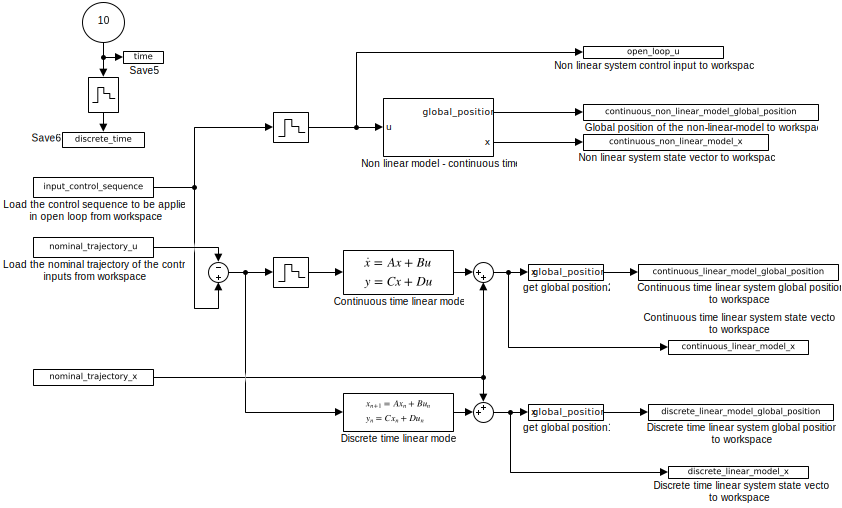
\includegraphics[width=\textwidth]{figures/simu_model.pdf}
	\caption{Simulink model for the simulation}
	\label{fig:simu_simulink}
\end{figure}
\begin{figure}[h]
	\centering
	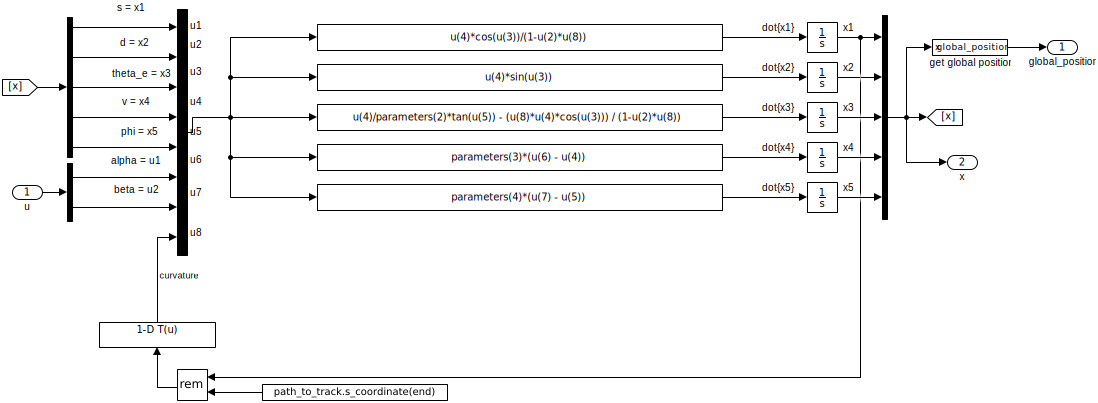
\includegraphics[width=\textwidth]{figures/nonlin.pdf}
	\caption{Modeled continuous-time nonlinear system.}
	\label{fig:simu_nonlin_simulink}
\end{figure}

\begin{table}[h]
	\centering
	\begin{tabular}{c|l}
	\hline
	\hline
	\textbf{Parameter} & \textbf{Value}\\
	\hline
	$L$ & $4$\\
	$\kappa (s)$ & $1e^{-10}$\\
	$\sigma_a$ & 5\\
	$\sigma_s$ & 1\\
	$v_{ref}$ & 3\\
	\hline
	\hline
	\end{tabular}
	\caption{Values for the system parameters used in the simulation}
	\label{tab:simu_param_values}
\end{table}
In order to investigate the behaviour of the systems, several experiments are carried out on the model.
Among all simulation the initial condition $\bb{x}_0$ is set to the initial value of the nominal trajectory 
\begin{equation}
	\bb{x}_0 = \bb{\bar{x}} (0) \, 
\end{equation}
and the system has no transience at $t = 0$. 
The initial state for the linearized systems $\bb{\tilde{x}}_0$ is always set to $0$ such that, again, the system has no transience at $t=0$.
Below, different simulations and experiments on the system are presented.

\paragraph{Exact Model in the Linear Subspace of the System: }
Consider again the system model $\mathbf{\dot{x}} = \mathbf{f}(\mathbf{x}, \mathbf{u}, t)$ in equations \eqref{eq:ss1} to \eqref{eq:ss5}.
The system is linear, as long as all the quantities ($x_2$, $x_3$ and $x_5$) stay constant, there is no heading error $x_3 = 0$ and the curvature $\kappa$ is zero.
In this case, the trigonometric functions in the differential equations behave as constants and the $\frac{1}{1- \kappa x_2}$ terms vanish.
On the nominal trajectory is no heading error and the curvature is very close ($\kappa = 1e^{-10}$) to zero.
Therefore, in this case, even the nonlinear system model behaves linearly.
The expectation is that there should be approximately no linearization error when applying $\bb{\bar{u}}$ as $\kappa$ is very small.
The same is true, when applying a varying reference speed as control input $u_1$ as long as the curvature is approximately zero and there is no error.
Figure~\ref{fig:ex1_ex2} shows two experiments, where the system is kept in the linear regime.
On the left, exactly the nominal input is applied as control input.
On the right, a step is applied in the reference velocity control signal $u_1$.
As the curvature is very small, the angular quantities are zero and the lateral error is zero, the system behaves approximately linearly and therefore the linearized models predict the system very well.
Even though, the step is rather large (from $3$ to $60$) the linearized systems show a good prediction of the states.
There are only very small errors in the angular state less than $2\cdot 10^{-8}$.
\begin{figure}[h!]
	\centering
	\begin{subfigure}{0.49\textwidth}
	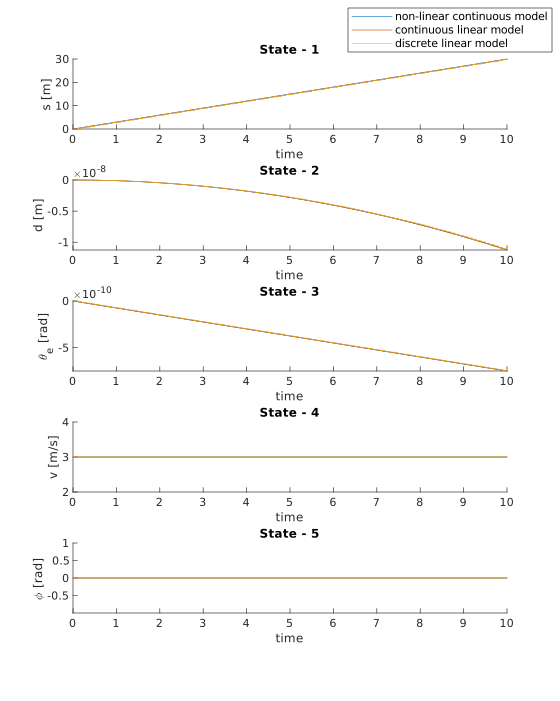
\includegraphics[width=\textwidth]{figures/ex1_states.pdf}
	\subcaption{Applying exactly the nominal input $\bb{\bar{u}}$.}
	\end{subfigure}
	\begin{subfigure}{0.49\textwidth}
	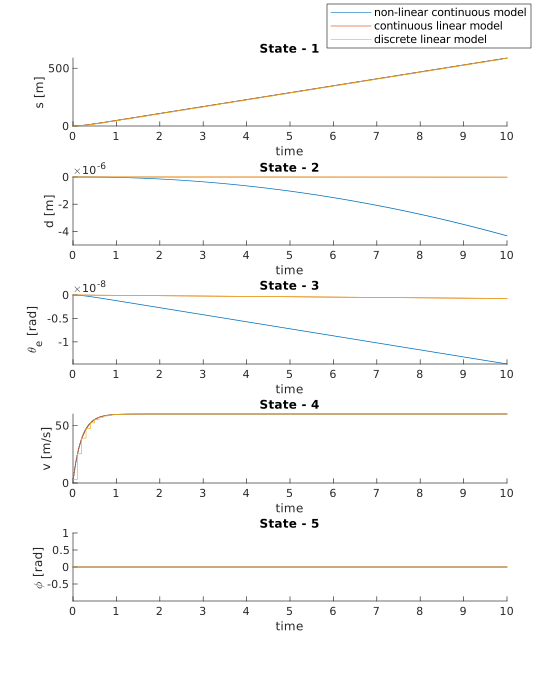
\includegraphics[width=\textwidth]{figures/ex2_states.pdf}
	\subcaption{Applying a step signal on the reference speed $u_1$.}
	\end{subfigure}
	\caption{Experiments in the linear regime of the model. On the left the nominal input is applied and on the right a (rather large) step in the speed is applied. As the system behaves linearly in this setting, the linearization error is very low. Note the small scale on the angle axes.}
	\label{fig:ex1_ex2}
\end{figure}

\paragraph{Going Nonlinear by Changing the Steering Angle: }
In the previous experiment it became obvious, that the linear approximation will work well, if the system stays in the linear subspace.
In order to excite the nonlinearities, the control input for the steering angle $u_2$ is changed.
Again, the initial state $\bb{x}_0$ is again set to the initial state of the nominal trajectory.
Figure~\ref{fig:ex345} shows the results for three different speeds with the same constant steering angle input of $u_2 = \frac{\pi}{6}$.
For low speeds (Figure~\ref{fig:ex3} and Figure~\ref{fig:ex4}) both, the continuous-time and discrete-time linear models overestimate the curvature of the path traced out by the vehicle.
On the other hand, for higher speeds as in Figure~\ref{fig:ex5} the linearized models underestimate the curvature.

\begin{figure}[h]
	\centering
	\begin{subfigure}{0.32\textwidth}
		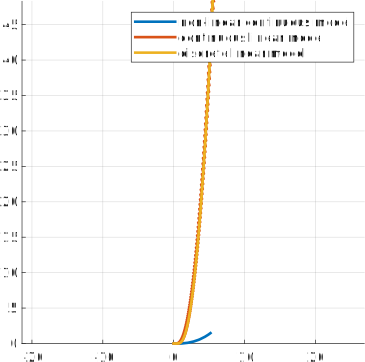
\includegraphics[width=\textwidth]{figures/ex1_4_3.pdf}
		\subcaption{$u_1 = 0.5$, $u_2 = \frac{\pi}{6}$}\label{fig:ex3}
	\end{subfigure}
	\begin{subfigure}{0.32\textwidth}
		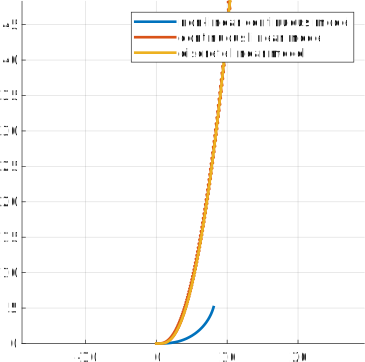
\includegraphics[width=\textwidth]{figures/ex1_4_4.pdf}
		\subcaption{$u_1 = 1$, $u_2 = \frac{\pi}{6}$}\label{fig:ex4}
	\end{subfigure}
	\begin{subfigure}{0.32\textwidth}
		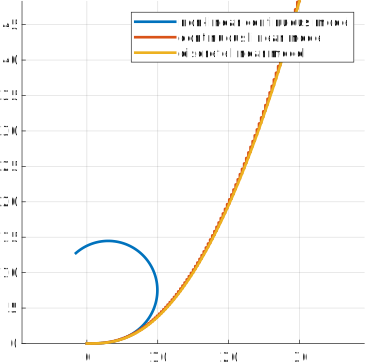
\includegraphics[width=\textwidth]{figures/ex1_4_5.pdf}
		\subcaption{$u_1 = 3$, $u_2 = \frac{\pi}{6}$}\label{fig:ex5}
	\end{subfigure}
	\caption{Setting the steering angle to $\frac{\pi}{6}$ leads to no longer good approximation of the system by the linear models. For different speeds the path is either more or less curved.}
	\label{fig:ex345}
\end{figure}

\paragraph{Settings for Very Poor Linear Approximation: }
Given the intuition from the previous when the model underestimates and when is overestimates the curvature, further experiments can be designed where the approximation is very poor. 
The resulting paths for these experiments are summarized in Figure~\ref{fig:ex6789}.

In Figure~\ref{fig:ex8} the steering angle is kept constant and the speed is switched from low to high after half time. 
As curvature of the linearly approximated path depends on the speed of the car, the curvature of the path traced out by the linear models changes upon changing the speed while the curvature of the nonlinear vehicle does not.

Figure~\ref{fig:ex7} shows a path, where the vehicle goes back and forth on the same circle-segment with a constant magnitude in speed and a constant steering angle.
Only the sign of the speed is flipped after half the time.
While the "nonlinear vehicle" comes back where is started, the "linear vehicles" go somewhere completely else.

The remaining figures show a flip in sign of the steering angle and both in steering angle and speed, respectively.
In both settings the magnitudes of the steering angle and the speed are kept constant and only the signed are flipped at half the time.

\begin{figure}[h]
	\centering
	\begin{subfigure}{0.49\textwidth}
		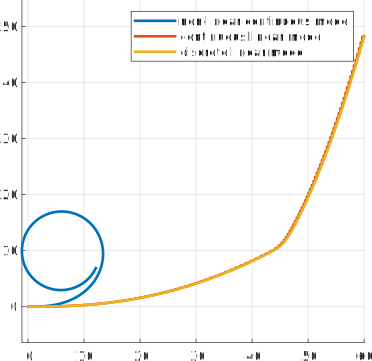
\includegraphics[width=\textwidth]{figures/ex1_4_8.pdf}
		\subcaption{Traveling on a curve with constant curvature at two different speeds.}\label{fig:ex8}
	\end{subfigure}
	\begin{subfigure}{0.49\textwidth}
		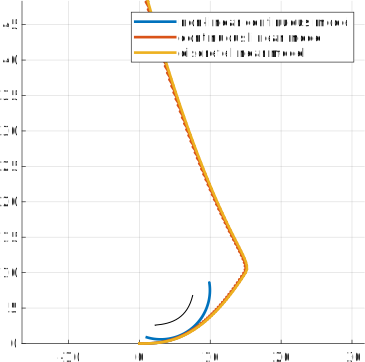
\includegraphics[width=\textwidth]{figures/ex1_4_7.pdf}
		\subcaption{Going back and forth on the same curve with the same steering angle and same absolute speed, but changing the sign of speed.}\label{fig:ex7}
	\end{subfigure}
	\begin{subfigure}{0.49\textwidth}
		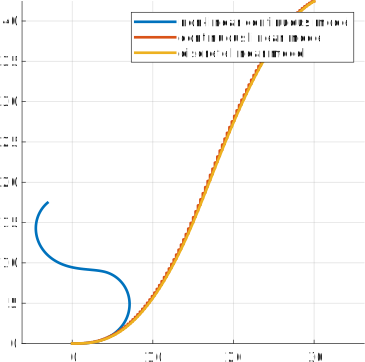
\includegraphics[width=\textwidth]{figures/ex1_4_6.pdf}
		\subcaption{Traveling at constant speed and flipping the sign of the steering angle rapidly.}\label{fig:ex6}
	\end{subfigure}
	\begin{subfigure}{0.49\textwidth}
		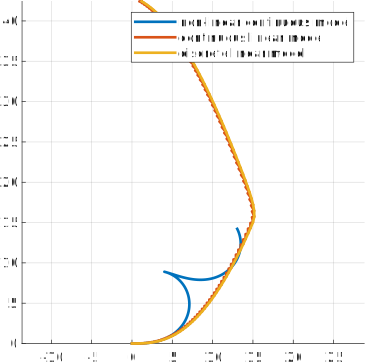
\includegraphics[width=\textwidth]{figures/ex1_4_9.pdf}
		\subcaption{Turning the vehicle by going first forward and then backward with flipped sign in the steering angle.}\label{fig:ex9}
	\end{subfigure}
	\caption{Control input settings, where the linear approximation is very wrong.}
	\label{fig:ex6789}
\end{figure}

\subsection{Summary of Observations}
The farer we are from the reference trajectory, the wronger the outcome of the linear model. 
Especially, changes of the steering angle lead to an erroneous result.
As can be seen in Figure~\ref{fig:ex6789}, the errors of the states are also coupled for the linear approximation.
For instance, the same steering angle leads to different (wrong) headings dependent of the speed.